\chapter{Modelação de Interfaces}

\section{Efectuar Login}
\begin{figure}[!htbp]
\centering
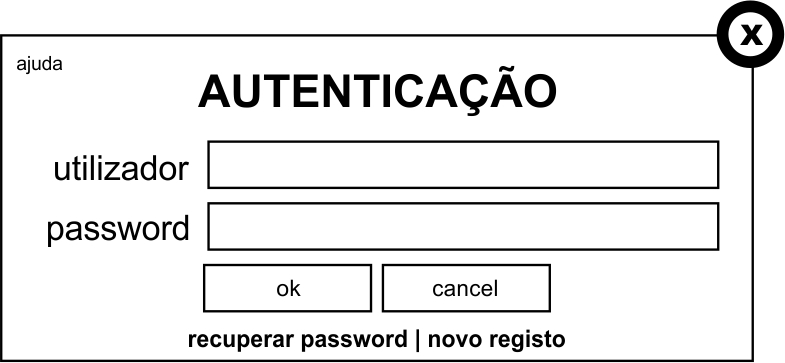
\includegraphics{imagens/login_i.jpg}
\caption{Interface: Login}
\label{fig:login_i}
\end{figure}


\clearpage
\section{Inscrever em Momento de Avaliação}

\begin{figure}[!htbp]
\centering
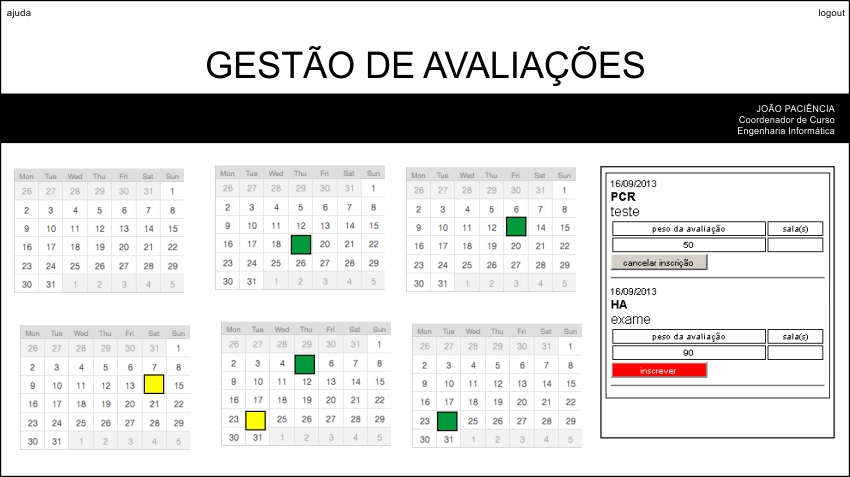
\includegraphics{imagens/inscrever_cancelar_inscricao_i.jpg}
\caption{Interface: Efectuar ou Cancelar Inscrição em Momento de Avaliação}
\label{fig:inscricao_avaliacao_i}
\end{figure}


\clearpage
\section{Marcar e Cancelar Momento de Avaliação}

\begin{figure}[!htbp]
\centering
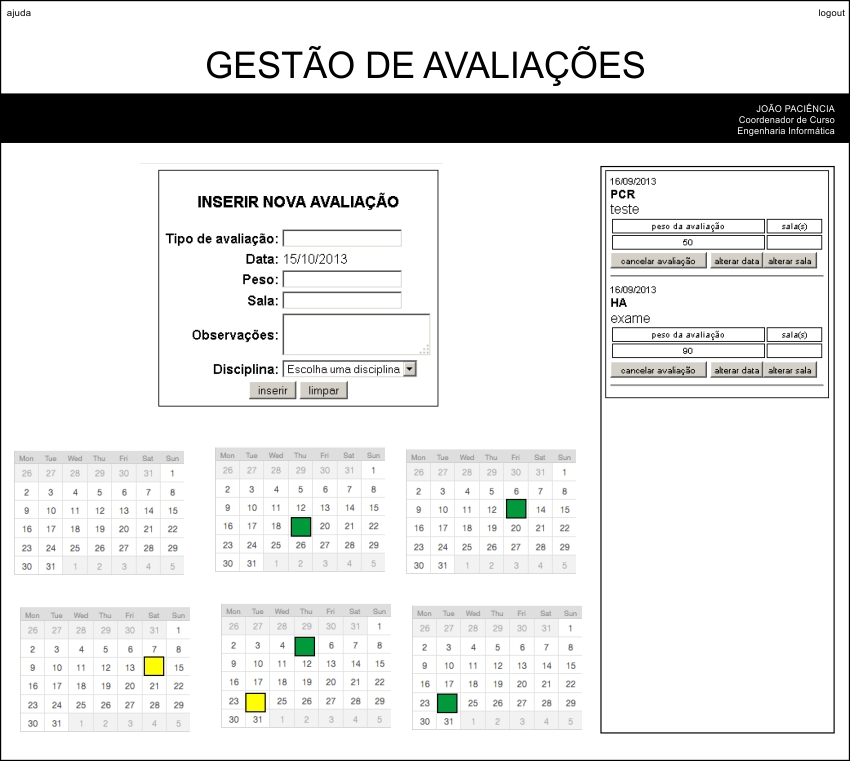
\includegraphics{imagens/nova_avaliacao_i.jpg}
\caption{Interface: Marcar Novo Momento de Avaliação}
\label{fig:nova_avaliacao_i}
\end{figure}


\clearpage
\section{Validar e Cancelar Validação de Momentos de Avaliação}

\begin{figure}[!htbp]
\centering
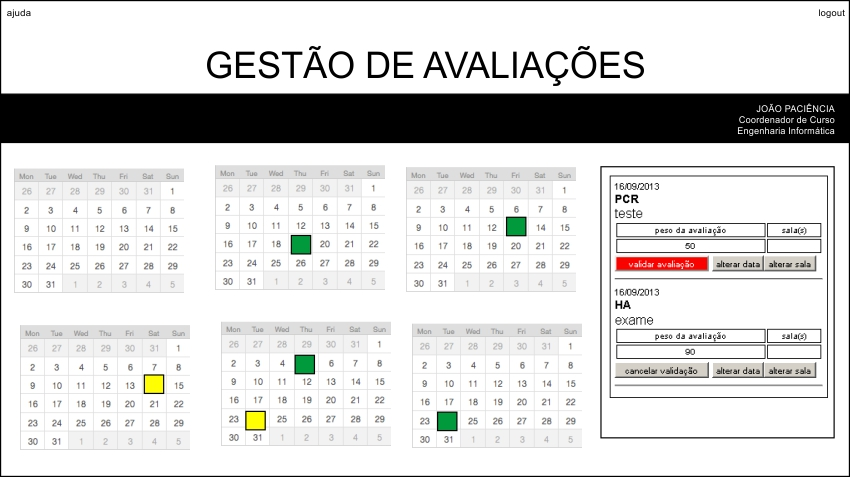
\includegraphics{imagens/validar_avaliacao_i.jpg}
\caption{Interface: Validar ou Cancelar Validação de Momento de Avaliação}
\label{fig:validar_avaliacao_i}
\end{figure}


\clearpage
\section{Listar Momentos de Avaliação}